\chapter{As plantas ao nosso redor}\label{ch:g1:plants-around-us}

Uma margarida no gramado, o musgo no muro, o castanheiro grandão do
pátio da escola: nenhum deles vai sair correndo, e mesmo assim todos
estão vivos. As \omterm{def:g1:plants-around-us:plant}{plantas} são os \omterm{def:g1:living-or-not:living}{seres vivos} quietos --- elas nascem,
se alimentam e crescem, às vezes por centenas de anos, sem nunca
sair do lugar.

\section{As plantas são seres vivos}

\begin{definition}[Planta]\label{def:g1:plants-around-us:plant}
Uma \emph{planta}\index{planta} é um \omterm{def:g1:living-or-not:living}{ser vivo} que fica preso ao chão
e fabrica o próprio alimento usando a luz. O capim, as margaridas, o
pé de tomate e as \omterm{def:g1:plants-around-us:tree}{árvores} são plantas. Quase todas as plantas são
verdes.
\end{definition}

\begin{example}[A margarida está viva]\label{ex:g1:plants-around-us:daisy}
Confira os sinais da vida numa margarida: ela nasceu de uma semente;
ela se alimenta --- com a água da terra e a luz do céu; ela cresce;
ela faz sementes que viram margaridas novas; ela morre na geada.
Todos os sinais estão lá. A margarida está tão viva quanto o gato
--- só que bem mais quietinha.
\end{example}

\begin{omfigure}
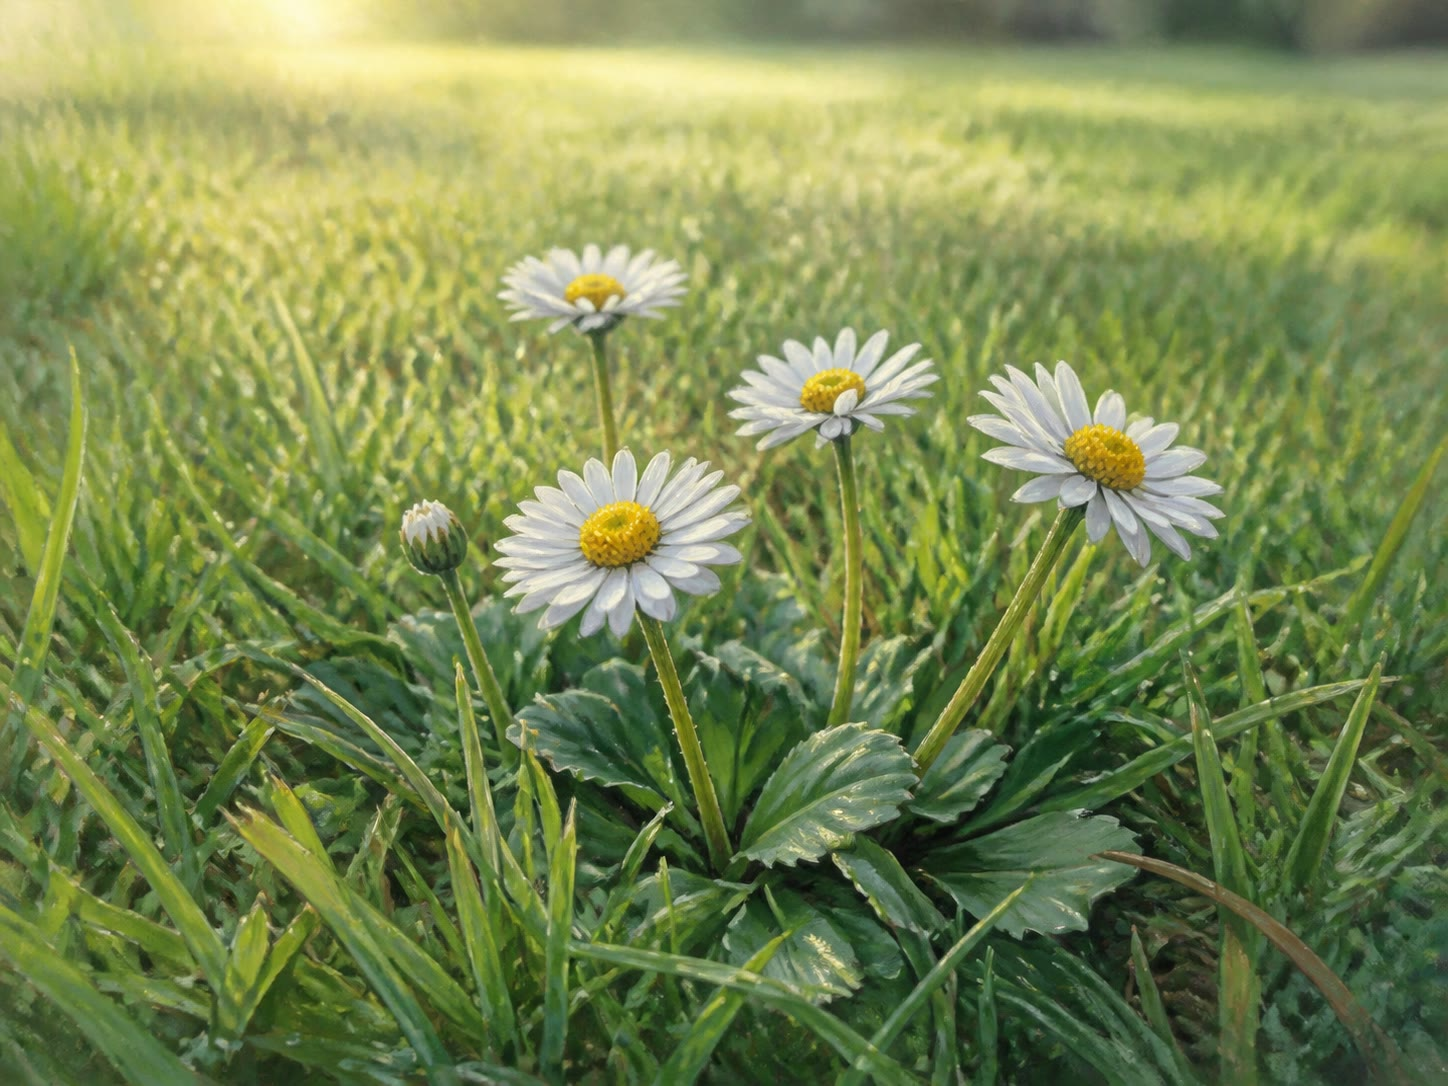
\includegraphics[width=0.58\linewidth]{images/book1/ai/g1-plants-daisy.jpg}

{\small Margaridas no gramado: nascidas de sementes, alimentando-se
de luz e água, vivas em silêncio.}
\end{omfigure}

\begin{remark}[Vivo sem correr]\label{rem:g1:plants-around-us:still}
As \omterm{def:g1:plants-around-us:plant}{plantas} não andam, mas também não ficam completamente paradas. Um
girassol se vira para acompanhar a luz durante o dia, e uma \omterm{def:g1:plants-around-us:plant}{planta} no
peitoril da janela vai se inclinando devagarinho para a janela. As
\omterm{def:g1:plants-around-us:plant}{plantas} se movem \emph{crescendo} --- devagar demais para os nossos
olhos, rápido o bastante para uma semana de observação.
\end{remark}

\section{As partes de uma planta}

\begin{definition}[Partes de uma planta]\label{def:g1:plants-around-us:parts}
Uma \omterm{def:g1:plants-around-us:plant}{planta} com flor tem quatro partes principais:
\begin{enumerate}
  \item a \emph{raiz}\index{raiz}, escondida na terra, que segura a
        \omterm{def:g1:plants-around-us:plant}{planta} no lugar e bebe a água;
  \item o \emph{caule}\index{caule}, que deixa a \omterm{def:g1:plants-around-us:plant}{planta} em pé e leva
        a água até as folhas;
  \item as \emph{folhas}\index{folha}, chatas e verdes, que captam a
        luz;
  \item a \emph{flor}\index{flor}, que vai fazer as sementes.
\end{enumerate}
\end{definition}

\begin{omfigure}
\begin{tikzpicture}
  \node[anchor=south west, inner sep=0] (img) at (0,0)
    {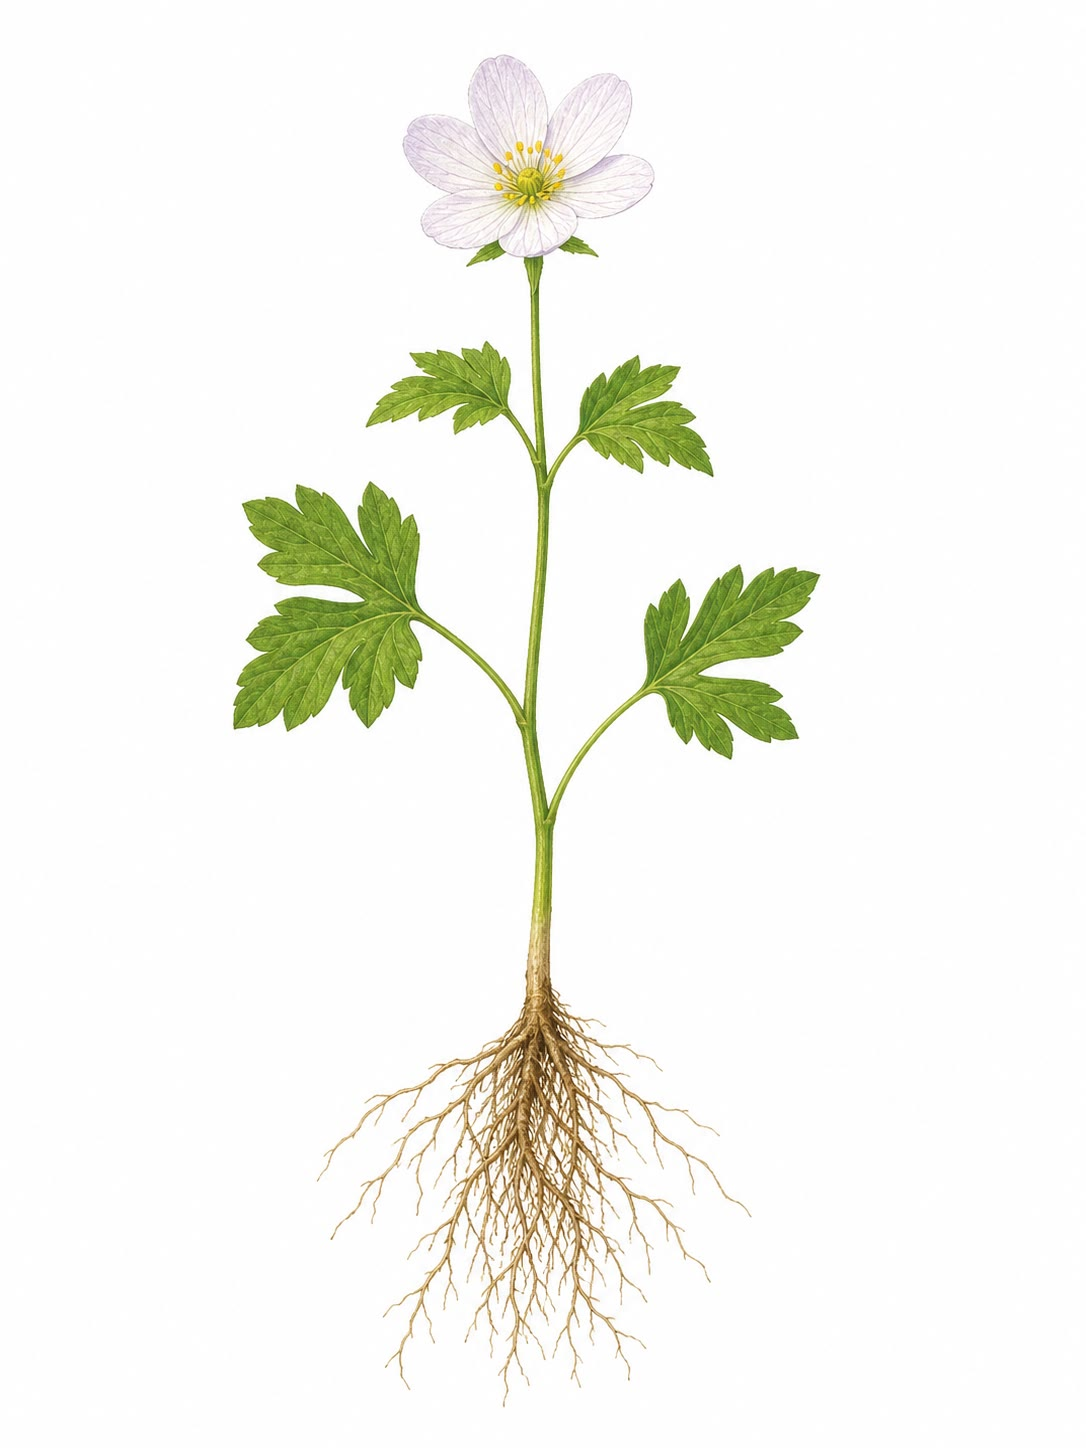
\includegraphics[width=0.5\linewidth]{images/book1/ai/fig-plant-uprooted.jpg}};
  \begin{scope}[x={(img.south east)}, y={(img.north west)},
      every node/.style={font=\small}]
    \draw[omDef, thick] (0.55,0.91) -- (0.74,0.93) node[right] {flor};
    \draw[omDef, thick] (0.68,0.57) -- (0.84,0.62) node[right] {folha};
    \draw[omDef, thick] (0.51,0.33) -- (0.74,0.36) node[right] {caule};
    \draw[omDef, thick] (0.58,0.13) -- (0.78,0.16) node[right] {raízes};
  \end{scope}
\end{tikzpicture}

{\small As quatro partes de uma \omterm{def:g1:plants-around-us:plant}{planta} com \omterm{def:g1:plants-around-us:parts}{flor}, arrancada inteira:
no chão, as \omterm{def:g1:plants-around-us:parts}{raízes} fazem o trabalho delas escondidas, debaixo da
terra.}
\end{omfigure}

\begin{example}[Arrancando um matinho]\label{ex:g1:plants-around-us:weed}
Arranque um matinho com jeitinho da terra fofa e molhada e você traz
para cima a parte escondida: um tufo de \omterm{def:g1:plants-around-us:parts}{raízes} claras, às vezes mais
comprido que toda a parte verde de cima. Agora dá para ler a \omterm{def:g1:plants-around-us:plant}{planta}
de baixo para cima: \omterm{def:g1:plants-around-us:parts}{raízes}, \omterm{def:g1:plants-around-us:parts}{caule}, \omterm{def:g1:plants-around-us:parts}{folhas} --- e, com sorte, uma \omterm{def:g1:plants-around-us:parts}{flor}.
\end{example}

\begin{definition}[Árvore]\label{def:g1:plants-around-us:tree}
Uma \emph{árvore}\index{árvore} é uma \omterm{def:g1:plants-around-us:plant}{planta} grande cujo \omterm{def:g1:plants-around-us:parts}{caule} é
feito de madeira. Esse \omterm{def:g1:plants-around-us:parts}{caule} de madeira se chama
\emph{tronco}\index{tronco}; ele se divide em
\emph{galhos}\index{galho}, que carregam as \omterm{def:g1:plants-around-us:parts}{folhas}.
\end{definition}

\begin{example}[O castanheiro]\label{ex:g1:plants-around-us:tree}
O castanheiro do pátio tem o mesmo plano da margarida, só que maior
e mais duro: \omterm{def:g1:plants-around-us:parts}{raízes} debaixo da terra, um tronco no lugar de um \omterm{def:g1:plants-around-us:parts}{caule}
macio, \omterm{def:g1:plants-around-us:tree}{galhos} com milhares de \omterm{def:g1:plants-around-us:parts}{folhas} e, na primavera, \omterm{def:g1:plants-around-us:parts}{flores}. A
margarida vive um ano; o castanheiro pode viver mais de cem.
\end{example}

\section{Do que uma planta precisa}

\begin{proposition}[As necessidades de uma planta]\label{prop:g1:plants-around-us:needs}
Para viver e crescer, uma \omterm{def:g1:plants-around-us:plant}{planta} precisa de \emph{água}, de
\emph{luz} e de um lugar para as \omterm{def:g1:plants-around-us:parts}{raízes}, quase sempre a
\emph{terra}\index{terra}. Uma \omterm{def:g1:plants-around-us:plant}{planta} guardada no escuro, ou que
nunca é regada, murcha e morre.
\end{proposition}
\admitted

\begin{example}[A planta esquecida]\label{ex:g1:plants-around-us:wilt}
Esqueça de regar a \omterm{def:g1:plants-around-us:plant}{planta} da sala antes das férias: as \omterm{def:g1:plants-around-us:parts}{folhas} dela
ficam caídas, moles e tristes --- ela murcha. Regue a \omterm{def:g1:plants-around-us:plant}{planta} e,
poucas horas depois, as \omterm{def:g1:plants-around-us:parts}{folhas} voltam a ficar em pé. A água era a
necessidade que faltava.
\end{example}

\begin{method}[Cuidar de uma planta]\label{met:g1:plants-around-us:care}
\begin{enumerate}
  \item Ponha o vaso onde a luz do dia chega;
  \item regue a terra quando ela estiver seca ao toque --- não a
        toda hora, porque as \omterm{def:g1:plants-around-us:parts}{raízes} também precisam de ar;
  \item não arranque as \omterm{def:g1:plants-around-us:parts}{folhas}: elas são as captadoras de luz da
        \omterm{def:g1:plants-around-us:plant}{planta};
  \item tenha paciência: uma \omterm{def:g1:plants-around-us:plant}{planta} responde em dias, não em minutos.
\end{enumerate}
\end{method}

\begin{remark}[As plantas alimentam todo mundo]\label{rem:g1:plants-around-us:food}
As \omterm{def:g1:plants-around-us:plant}{plantas} são importantes para todos os \omterm{def:g1:animals-around-us:animal}{animais}. O caracol come a
alface, o sabiá come frutinhas, nós comemos pão feito de trigo ---
uma \omterm{def:g1:plants-around-us:plant}{planta}. Até o gato, que não come alface, come \omterm{def:g1:animals-around-us:animal}{animais} que
comeram \omterm{def:g1:plants-around-us:plant}{plantas}. Sem as \omterm{def:g1:plants-around-us:plant}{plantas}, ninguém mais teria o que comer; um
capítulo mais adiante segue essas cadeias alimentares.
\end{remark}

\section{Exercícios}

\begin{exercise}[$\star$]\label{exo:g1:plants-around-us:1}
Diga as quatro partes de uma \omterm{def:g1:plants-around-us:plant}{planta} com \omterm{def:g1:plants-around-us:parts}{flor}, de baixo da terra até
o alto.
\end{exercise}

\begin{exercise}[$\star$]\label{exo:g1:plants-around-us:2}
Qual parte da \omterm{def:g1:plants-around-us:plant}{planta}: (a) bebe a água da terra? (b) capta a luz?
(c) vai fazer as sementes? (d) segura a \omterm{def:g1:plants-around-us:plant}{planta} em pé?
\end{exercise}

\begin{exercise}[$\star$]\label{exo:g1:plants-around-us:3}
A margarida nunca anda. Passe pelos sinais da vida e diga por que
mesmo assim ela é um \omterm{def:g1:living-or-not:living}{ser vivo}.
\end{exercise}

\begin{exercise}[$\star$]\label{exo:g1:plants-around-us:4}
Quais são os nomes especiais do \omterm{def:g1:plants-around-us:parts}{caule} da \omterm{def:g1:plants-around-us:tree}{árvore} e das partes que
carregam as \omterm{def:g1:plants-around-us:parts}{folhas} dela?
\end{exercise}

\begin{exercise}[$\star$]\label{exo:g1:plants-around-us:5}
Diga as três coisas de que uma \omterm{def:g1:plants-around-us:plant}{planta} precisa para viver, segundo a
\cref{prop:g1:plants-around-us:needs}.
\end{exercise}

\begin{exercise}[$\star$]\label{exo:g1:plants-around-us:6}
A \omterm{def:g1:plants-around-us:plant}{planta} da sala está com as \omterm{def:g1:plants-around-us:parts}{folhas} moles e caídas. O que
provavelmente foi esquecido? O que vai acontecer depois que ela
receber isso?
\end{exercise}

\begin{exercise}[$\star$]\label{exo:g1:plants-around-us:7}
Em que a margarida e o castanheiro são iguais? Em que duas coisas
eles são diferentes?
\end{exercise}

\begin{exercise}[$\star$]\label{exo:g1:plants-around-us:8}
Faça a experiência: ponha um pé de feijão (ou um potinho de agrião)
perto da janela e outro dentro de um armário escuro, e regue os
dois. Olhe depois de uma semana. Que diferença você espera, e qual
necessidade explica isso?
\end{exercise}

\begin{exercise}[$\star\star$]\label{exo:g1:plants-around-us:9}
O Léo diz: ``As \omterm{def:g1:plants-around-us:plant}{plantas} não são vivas de verdade --- elas nunca
fazem nada.'' Dê a ele duas coisas que uma \omterm{def:g1:plants-around-us:plant}{planta} faz, devagar mas
sem falhar, a partir da \cref{rem:g1:plants-around-us:still} e do
\cref{ex:g1:plants-around-us:daisy}.
\end{exercise}

\begin{exercise}[$\star\star$]\label{exo:g1:plants-around-us:10}
A cenoura é laranja e cresce debaixo da terra. Olhando a figura das
partes da \omterm{def:g1:plants-around-us:plant}{planta}, qual parte do pé de cenoura você acha que a gente
come? Que pista a expressão ``debaixo da terra'' dá?
\end{exercise}
